% Created 2019-07-17 三 21:45
% Intended LaTeX compiler: pdflatex
\documentclass[11pt]{article}
\usepackage[utf8]{inputenc}
\usepackage[T1]{fontenc}
\usepackage{graphicx}
\usepackage{grffile}
\usepackage{longtable}
\usepackage{wrapfig}
\usepackage{rotating}
\usepackage[normalem]{ulem}
\usepackage{amsmath}
\usepackage{textcomp}
\usepackage{amssymb}
\usepackage{capt-of}
\usepackage{hyperref}
\author{channing}
\date{\today}
\title{}
\hypersetup{
 pdfauthor={channing},
 pdftitle={},
 pdfkeywords={},
 pdfsubject={},
 pdfcreator={Emacs 26.2 (Org mode 9.1.9)}, 
 pdflang={English}}
\begin{document}

\tableofcontents

\section{敏捷开发}
\label{sec:org9ae2bea}
\subsection{敏捷联盟宣言}
\label{sec:org2c71d19}
\begin{description}
\item[{个体和交互胜过过程和工具}] 人是获得成功的最为重要的因素。如果团队中没有优秀的成员,那么就是使用好的过程也不能从失败中挽救项目。
但是,孬的过程却可以使最优秀的团队成员推动盗用。如果不能作为一个团队进行工作,那么即使拥有最优秀的成员也一样会惨败。
\item[{可以工作的软件胜过面面俱到的文档}] 对于团队来说,编写并维护一份系统原理和结构方面的文档将总是一个好主意,
但是那套文档应该是短小并且主题突出的。
\item[{客户合作胜过合同谈判}] 成功的项目需要有序、频繁的客户反馈。不是依赖于合同或者关于工作的陈述,
而是让软件的客户和开发团队密切地在一起工作,并尽量经常地提供反馈。
\item[{响应变化胜过遵循计划}] 计划不能考虑得过远。道德,商务环境很可能会变化,这会会引起需求的变动。其次,一旦客户看到系统开始运作,
他们很可能会改变需求。最后,即使我们熟悉需求,并且确信它们不会发迹,我们仍然不能很好地估算出开发它们需要的时间。
\end{description}
\subsection{敏捷开发的原则}
\label{sec:org7816e8f}
\begin{enumerate}
\item 我们最优先要做的是通过尽早的、待续的交付有价值的软件来使客户满意
\item 即使到了开发的后期,也欢迎改变需求。敏捷过程利用变化来为客户创造竞争优势。
\item 经常性地交付可以工作的软件,交付的间隔可以从几周到几个朋,交付的时间间隔越短越好。
\item 在整个项目开发期间,业务人员和开发人员必须天天都在一起工作。
\item 围绕被激励起来的个人来构建项目。给他们提供所需要的环境和支持,并且信任他们能够完成工作。
\item 在团队内部,最具有效果并且富有效率的传递信息的方法,就是面对面的交谈。
\item 工作的软件是首要的进度度量标准。
\item 敏捷过程提倡可持续的开发速度。责任人、开发者和用户应该能够保持一个长期的、恒定的开发速度。
\item 不能地关注优秀的技能和好的设计会增强敏捷能力。
\item 简单──使未完成的工作最大化的──是根本的。
\item 最好的构架、需求和设计出自于自组织的团队。
\item 每隔一定时间,团队会在如何才能更有效地工作方面进行反省,然后相应地对自己的行为进行调整。
\end{enumerate}

\section{极限编程}
\label{sec:org88069c2}
极限编程是敏捷方法中最著名的一个。它由一系列简单却互相依赖的实践组成。这些实践结合在一起形成了一个胜于部分结合的整体。

\begin{enumerate}
\item 客户作为团队成员
\item 用户素材
\item 短交付周期
\item 验收测试
\item 结对编程
\item 测试驱动的开发方法
\item 集体所有权
\item 持续集成
\item 可持续的开发速度
\item 开放的工作空间
\item 计划游戏
\item 简单的设计
\item 重构
\item 隐喻
\end{enumerate}

\section{设计原则}
\label{sec:org68e07e2}
\subsection{单一职责原则(SRP)}
\label{sec:orga7caf47}
\begin{description}
\item[{定义}] 就一个类而言,应该仅有一个引起它变化的原因。
\item[{什么是职责}] 在SRP中,我们把职责定义为“变化的原因”。如果你能够想到多于一个的动机去改变一个类,那么这个类就具有多于一个的职责。
有时,我们很难注意到这一点。我们习贯于以组的形式去考虑职责。
\end{description}
\subsection{开放——封闭原则(OCR)}
\label{sec:org839b037}
\begin{description}
\item[{定义}] 软件实体(类、模块、函数等等)应该是可以扩展的,但是不可修改的。
\end{description}

\subsubsection{遵循开放──封闭原则设计出的模块具有两个主要的特征}
\label{sec:org375308c}
\begin{description}
\item[{对于扩展开放}] 模块的行为是可以扩展的。当应用的需求改变时,我们可以对模块进行扩展,使其具有满足那些改变的新行为。
\item[{对于更改是封闭的}] 对模块行为进行扩展时,不必改动模块的源代码或者二进制代码。模块的二进制可执行版本,
无论是可链接的库、DLL或者Java的.jar文件,都无需改动。
\end{description}
\subsection{Liskov替换原则(LSP)}
\label{sec:org447d111}
\begin{description}
\item[{定义}] 子类型必须能够替换掉它们的基类型。
\item[{相对满足}] 事实上,一个模型,如果孤立地看,里氏替换并不具有真正意义上的有效性,模型的有效性只能通过它的客户程序来表现。
\item[{启发示方法}] \begin{enumerate}
\item 在派生类中存在退化函数并不总是表示违反了LSP,但是当这种情况存在时,
\item 当在派生类中添加了其基类不会抛出的异常时,如果基类的使用者不期望这些异常,那么把它们添加到派生类的方法中应付导致不可替换性。
此时要遵循LSP,要么就必须改变使用者的期望,要么派生类就不应该抛出这些异常。
\end{enumerate}
\end{description}
\subsection{依赖倒置原则(DIP)}
\label{sec:orgc9543b9}
\begin{description}
\item[{定义}] \begin{itemize}
\item 高层模块不应该依赖于低层模块,二者都应该位赖于抽象。
\item 抽象不应该依赖于细节,细节应该依赖于抽象。
\end{itemize}
\item[{解释}] 请注意这里的倒置不仅仅是依赖关系的倒置,它也是接口所有权的倒置。当应用了DIP时,往往是客户拥有抽象接口,
而它们的服务者则从这些抽象接口派生。
\item[{启发示规则──领事于抽象}] \begin{itemize}
\item 任何变量都不应该持有一个指向具体类的指针或者引用。
\item 任何类都不应该从具体类派生。
\item 任何方法都不应该覆写它的任何基类中的已经实现了的方法。
\item 如果一个具体类不太会改变,并且也不会创建其他类似的派生类,那么依赖于它并不会造成损害。
\end{itemize}
\end{description}
\subsection{接口隔离原则(ISP)}
\label{sec:org7347ce9}
\begin{description}
\item[{定义}] 不应该强制客户领事于它们不用的方法。如果强迫客户程序依赖于那些它们不使用的方法,
那么这些客户程序就面临着由于这些未使用方法的改变所带来的变更,这无意中导致了所有客户程序之间的耦合。
\end{description}
\section{设计模式}
\label{sec:org84b4395}
\subsection{Command模式和Active Object}
\label{sec:org07c5bac}
\subsubsection{Command模式的优点}
\label{sec:orgb099ef8}
\begin{enumerate}
\item 通过对命令概念的封装,可以解除系统的逻辑互联关系和实际连接的设备之前的耦合。
\item 另一个Command模式的常见用法是创建和执行事务操作。
\item 解耦数据和逻辑,可以将数据放在一个列表中,以后再进行实际的操作。
\end{enumerate}
\subsubsection{Active Object模式}
\label{sec:orgf50beff}
\begin{description}
\item[{描述}] Active Object模式是实现多线程控制的一项古老的技术。
控制核心对象维护了一个Command对象的链表。用户可以向链表中增加新的命令,或者调用执行动作,该动作只是遍历链表,执行并去除每个命令。
\item[{RTC任务}] 采用该技术的变体一去构建多线程系统已经是并且将会一直是一个很常见的实践。这种类型的线程被称为run-to-completion任务(RTC),
因为每个Command实例在下一个Command补全可以运行之前就运行完成了。RTC的名字意味着Command实例不会阻塞。
\item[{共享运行时堆栈}] Command实例一经运行就一定得完成的的赋予了RTC线程有趣的优点,寻就是它们共享同一个运行时堆栈。和传统的多线程中的线程不同,
不必为每个RTC线程定义或者分配各处的运行时堆栈。这在需要大量线程的内存受限系统中是一个强大的优势。
\end{description}
\subsection{Template Method模式和Strategy模式:继承和委托}
\label{sec:orgb134e05}
\subsubsection{Template Method模式}
\label{sec:orge515801}
\begin{description}
\item[{描述}] Template Method模式展示了面向对象编程上诸多经典重用形式中的一种。其中通用算法被放置在基类中,
并且通过继承在不同的具体上下文实现该通用算法。
\item[{代价}] 继承是一种非常强的关系,派生类不可避免地要和它们的基类绑定在一起。
\end{description}
\subsubsection{Strategy模式}
\label{sec:org706cc45}
\begin{description}
\item[{描述}] Strategy模式使用了一种非常不同的方法来倒置通用算法和具体实现之间的依赖关系。不是将通用的应用算法放进一个抽象基类中,
而是将它放进一个具体类中,在该具体类中定义一个成员对象,该成员对象实现了实际需要执行的具体算法,
在执行通用算法时,把具体工作委托给这个成员对象的所实现的抽象接口去完成。
\end{description}
\subsubsection{对比}
\label{sec:orgaf31274}
\begin{description}
\item[{共同点}] Template Method模式和Strategy模式都可以用来分离高层的算法和的具体实现细节,都允许高速的算法独立于它的具体实现细节重用。
\item[{差异}] Strategy模式也允许具体实现细节独立于高层的算法重用,不过要惟一些额外的复杂性、内存以及运行时间开销作为代价。
\end{description}

\subsection{Facade模式和Mediator模式}
\label{sec:orgfa975e9}
\subsubsection{facade模式}
\label{sec:orgba62801}
\begin{description}
\item[{使用场景}] 当想要为一组具有复杂且全面的接口的对象提供一个简单且特定的接口时,可以使用Facade模式,如下图所示的场景。
\begin{figure}[htbp]
\centering
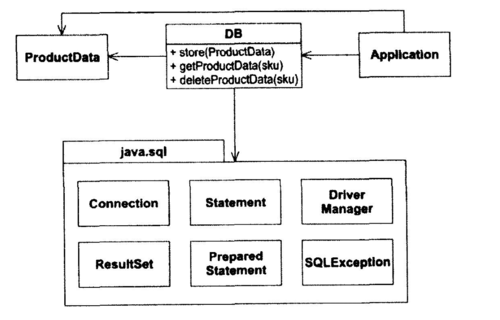
\includegraphics[width=.9\linewidth]{./dbFacade.png}
\caption{Facade模式封装数据库操作}
\end{figure}
\item[{基于约定}] 使用Facade模式意味着开发人员已经接受了所有数据库调用都要通过DB类的约定。如果任务一部分代码越过该Facade直接去访问java.sql,
那么就违反了该约定。基于约定,DB类成为了java.sql包的惟一代理。
\end{description}
\end{document}
